En esta sección concretamos en circuitos reales los conceptos abstractos de la sección anterior, justificando cada parte del circuito y la elección de sus componentes.
En la figura~\figref{fig:designed_circuit} puede verse nuestro circuito amplificador completo, incluyendo el punto de trabajo de cada transistor, es el circuito que se usó en cada una de las simulaciones para validar el circuito contra las especificaciones que se establecieron. En el circuito también se marcaron algunos ratings de componentes, potencias de resistores y tensiones de capacitores, los cuales se obtuvieron de las simulaciones, estos se especificaron y se usaron a la hora de armar el listado de componentes final, teniendo en cuenta también las tecnologías adecuadas para cada componente elegido.

\clearpage


\begin{figure}[H]
\centering
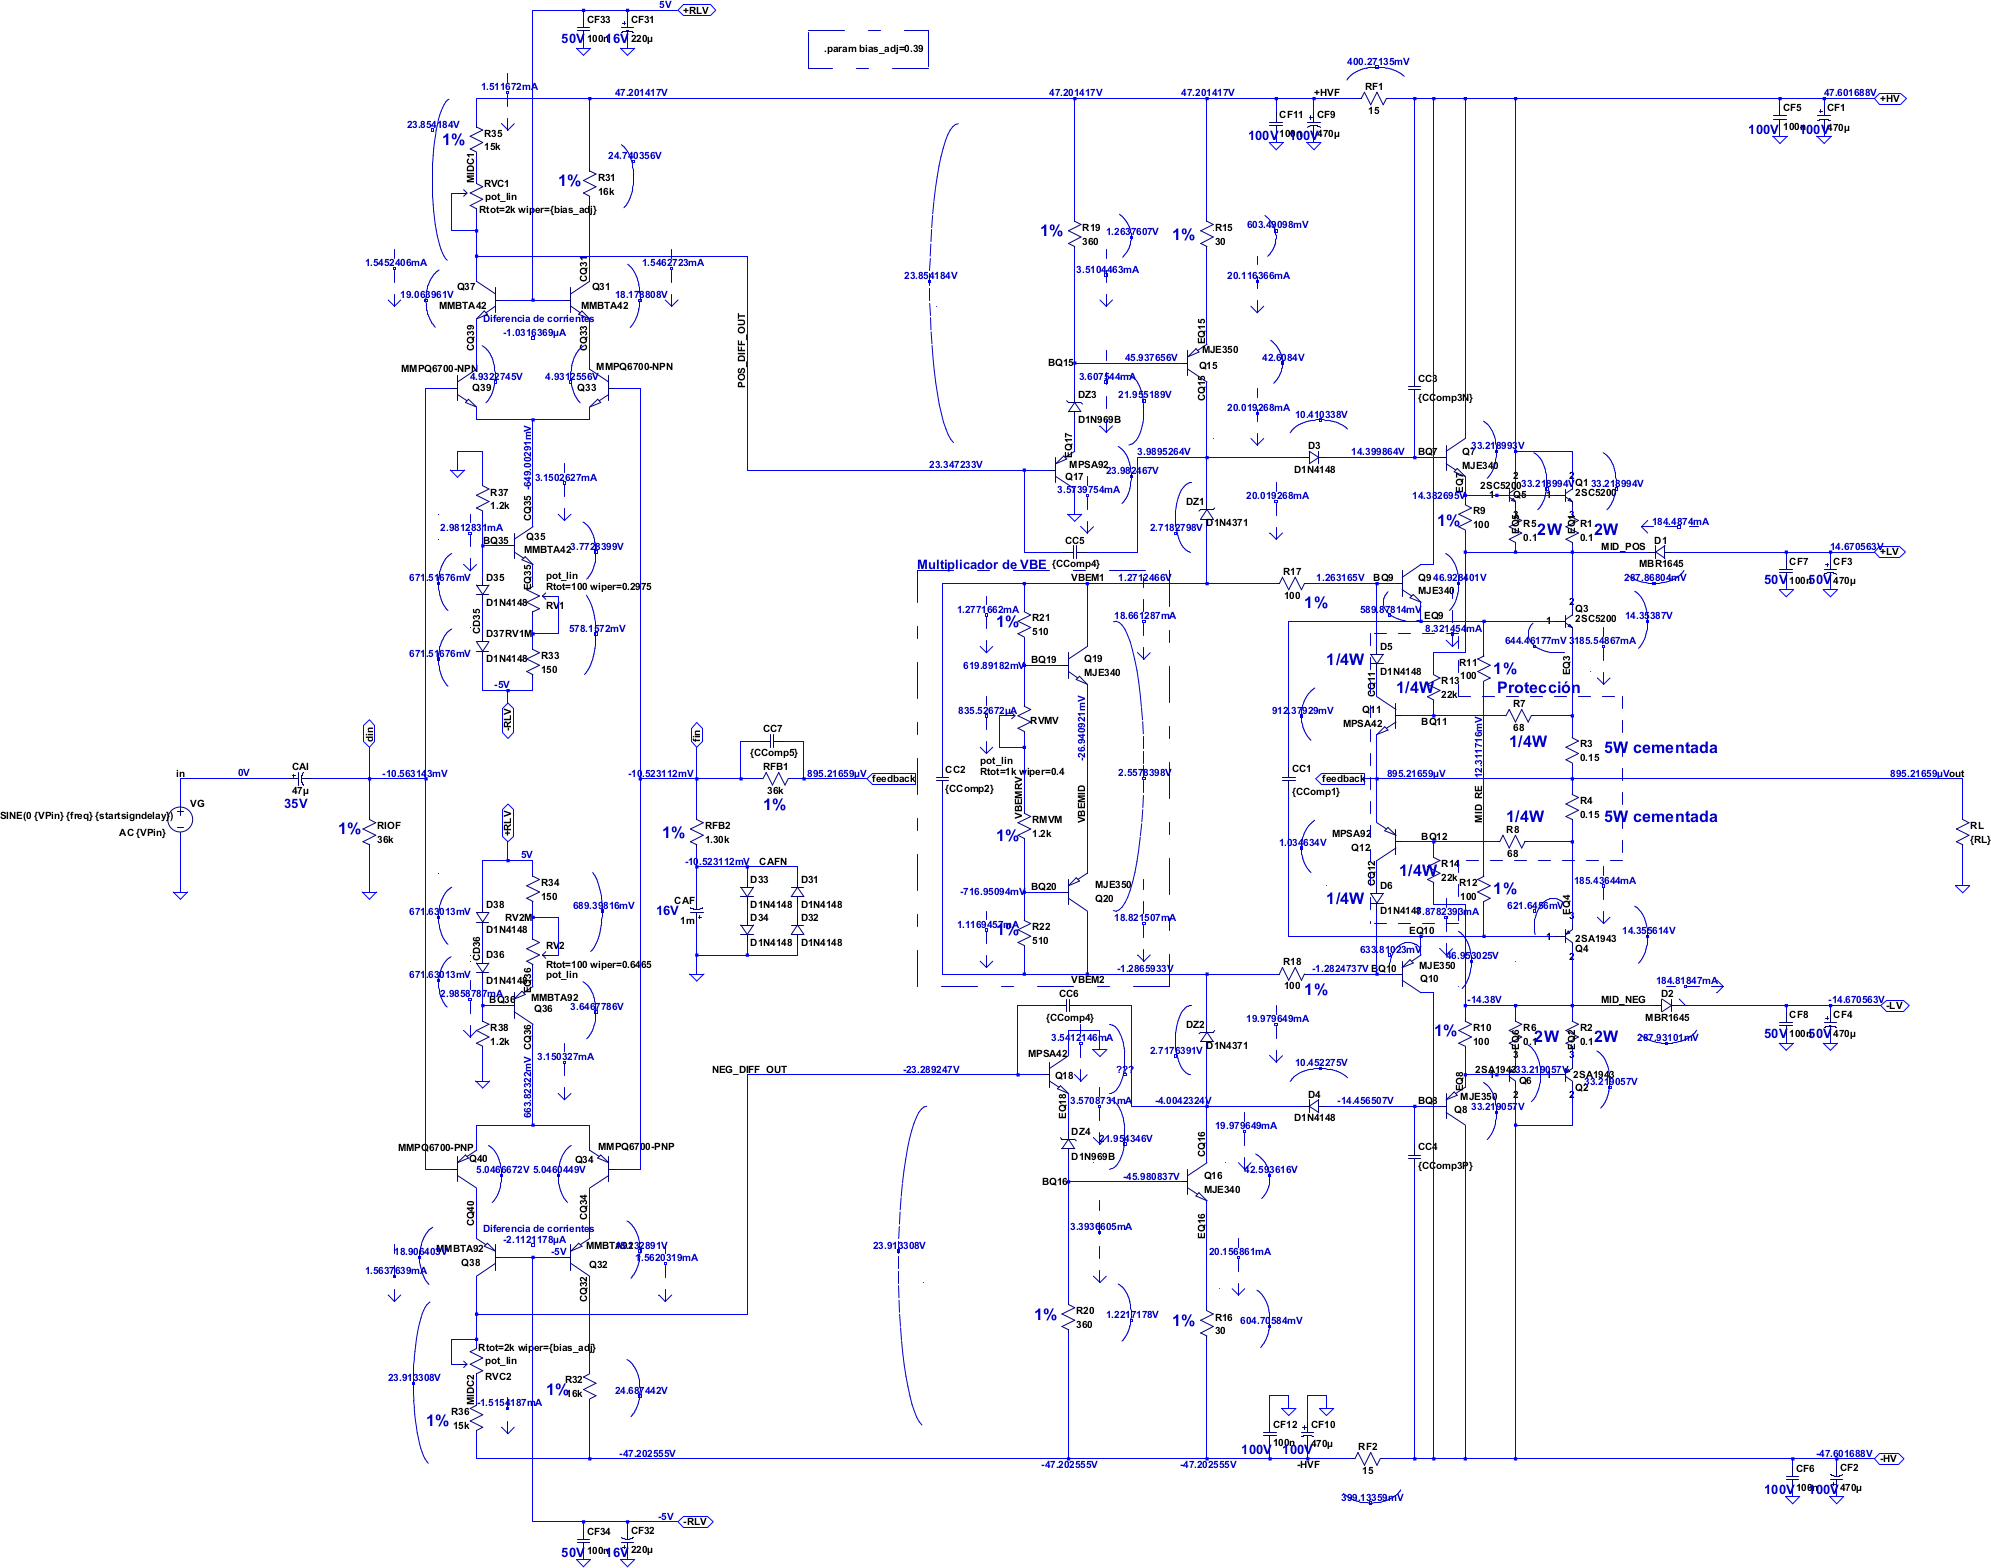
\includegraphics[width=0.9\paperwidth,angle=90,origin=c]{img/circuito.png}
\caption{Circuito Diseñado}
\label{fig:designed_circuit} 
\end{figure}

\clearpage


\subsection{Etapa de entrada}


Se usó doble par diferencial para mantener la simetría total y reducir la distorsión por armónicos pares, figura~\figref{fig:etapa-1}. Cada par se diseñó teniendo en cuenta que la tensión de salida de polarización debía ser estable, pues la segunda etapa no estará polarizada por una fuente de corriente. Por esto, los resistores de carga de los pares diferenciales ($R_{35}$, $RVC_{1}$ y $R_{36}$, $RVC_{2}$) son formadas por un resistor fijo de $15 \si[per-mode=symbol]{\kilo\ohm}$ y un preset multi-vuelta de $2 \si[per-mode=symbol]{\kilo\ohm}$, mucho menor que la resistencia dinámica de pequeña señal que le ofrece la segunda etapa ($\approx 60 \si[per-mode=symbol]{\kilo\ohm}$), dominando el paralelo. El ajuste de la polarización, consiste en ajustar primero la corriente de las fuentes de corriente y luego ajustar los presets de las cargas para lograr el punto deseado.
Por la misma razón, se consideró de particular importancia garantizar que las corrientes de polarización por las ramas del par se independicen de posibles variaciones en la segunda etapa o del riel. Los transistores $Q_{33}$~con~$Q_{39}$ y $Q_{34}$~con~$Q_{40}$, en configuración cascode combinados a $Q_{37}$~con~$Q_{31}$ y $Q_{38}$~con~$Q_{32}$ cumplen justamente la función de generar esta independencia.


\begin{wrapfigure}{R}{0.5\textwidth}
  \begin{center}
   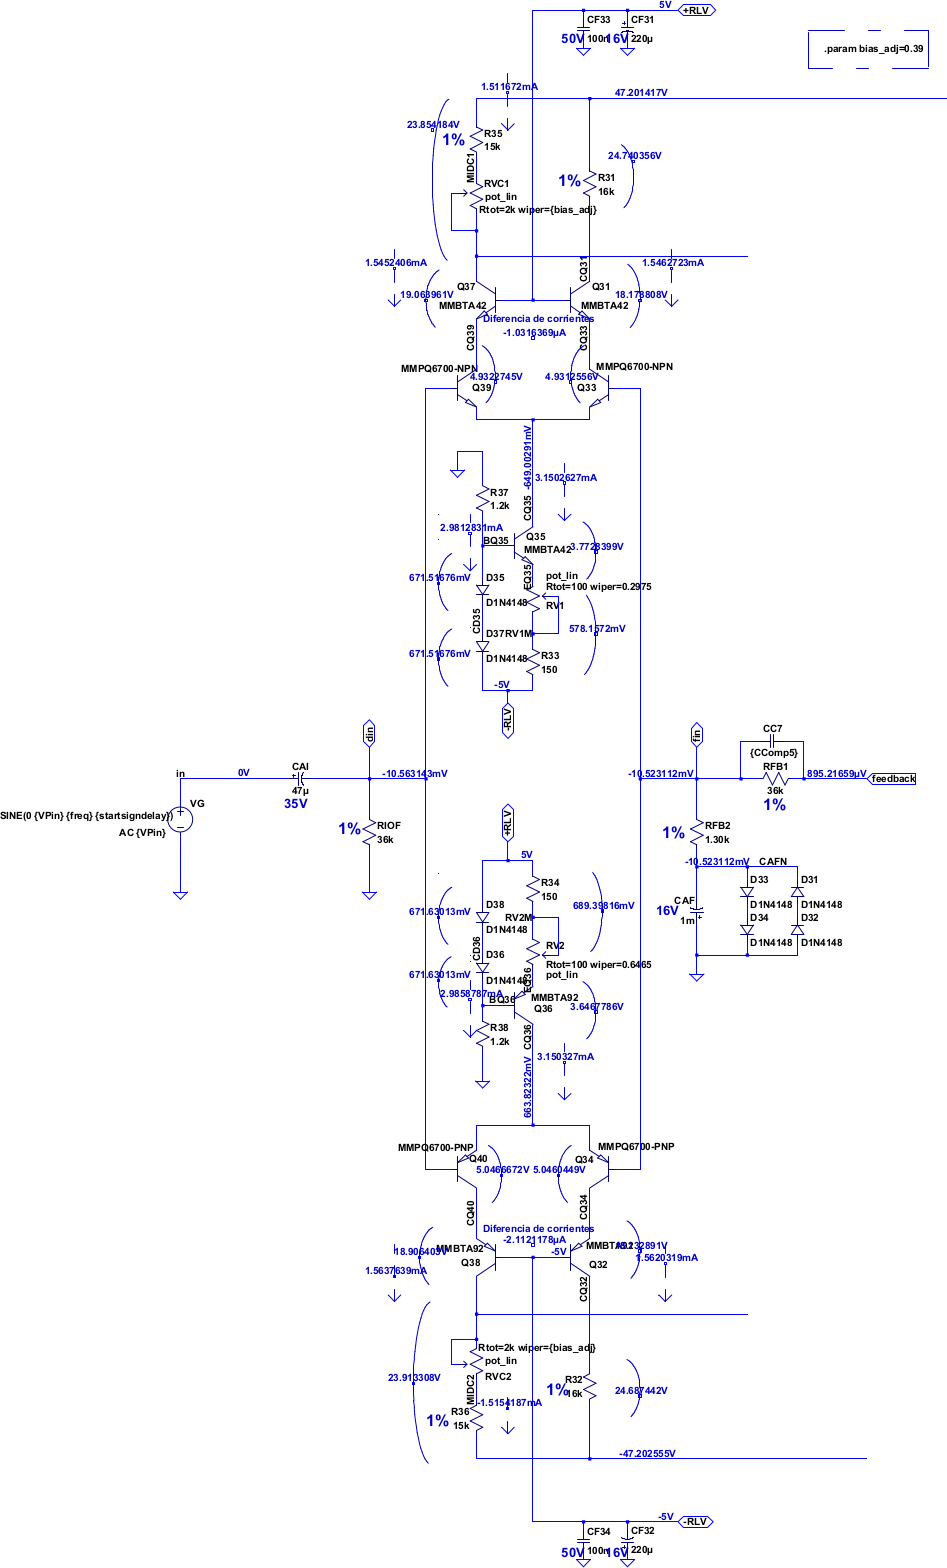
\includegraphics[width=0.4\textwidth]{img/etapa-1.png}
   \caption{Etapa primera del circuito diseñado.}
   \label{fig:etapa-1}
  \end{center}   
\end{wrapfigure}


Se polarizó cada rama con una corriente de $1.56 \si[per-mode=symbol]{\milli\ampere}$. Mayor corriente no generaría una mucho mayor amplificación de la etapa, pues, para mantener una tensión de salida fija habría sido necesario reducir la resistencia de carga en igual proporción. Esta corriente se generó con fuentes de corriente de $3.15 \si[per-mode=symbol]{\milli\ampere}$, se ajusta para que por los resistores de carga circulen $1.5 \si[per-mode=symbol]{\milli\ampere}$, logrando los $23.85 \si[per-mode=symbol]{\volt}$, independientes de la alimentación, que polarizan la segunda etapa. Los transistores de los pares diferenciales están formados cada uno por dos de los transistores de un array integrado, el \textbf{MMPQ6700}, de cuatro transistores, dos \textbf{NPN} y dos \textbf{PNP}, estos transistores como se mencionó tienen baja tensión de ruptura, pero el circuito elegido garantiza su operación segura, al ser integrados se tiene un grado alto de matcheo en sus características, esta característica se aprovecha para armar los diferenciales, dejando los base común de los cascodes a ser implementados por transistores complementarios discretos del tipo \textbf{MMBTA42}/\textbf{MMBTA92}, que son las versiones \textbf{SMD} de los conocidos transistores complementarios \textbf{MPSA42}/\textbf{MPSA92}, generalmente usados en amplificadores de potencia justamente por sus altas tensiones de ruptura y buenas características para audio.



%\begin{figure}[H]
%\centering
%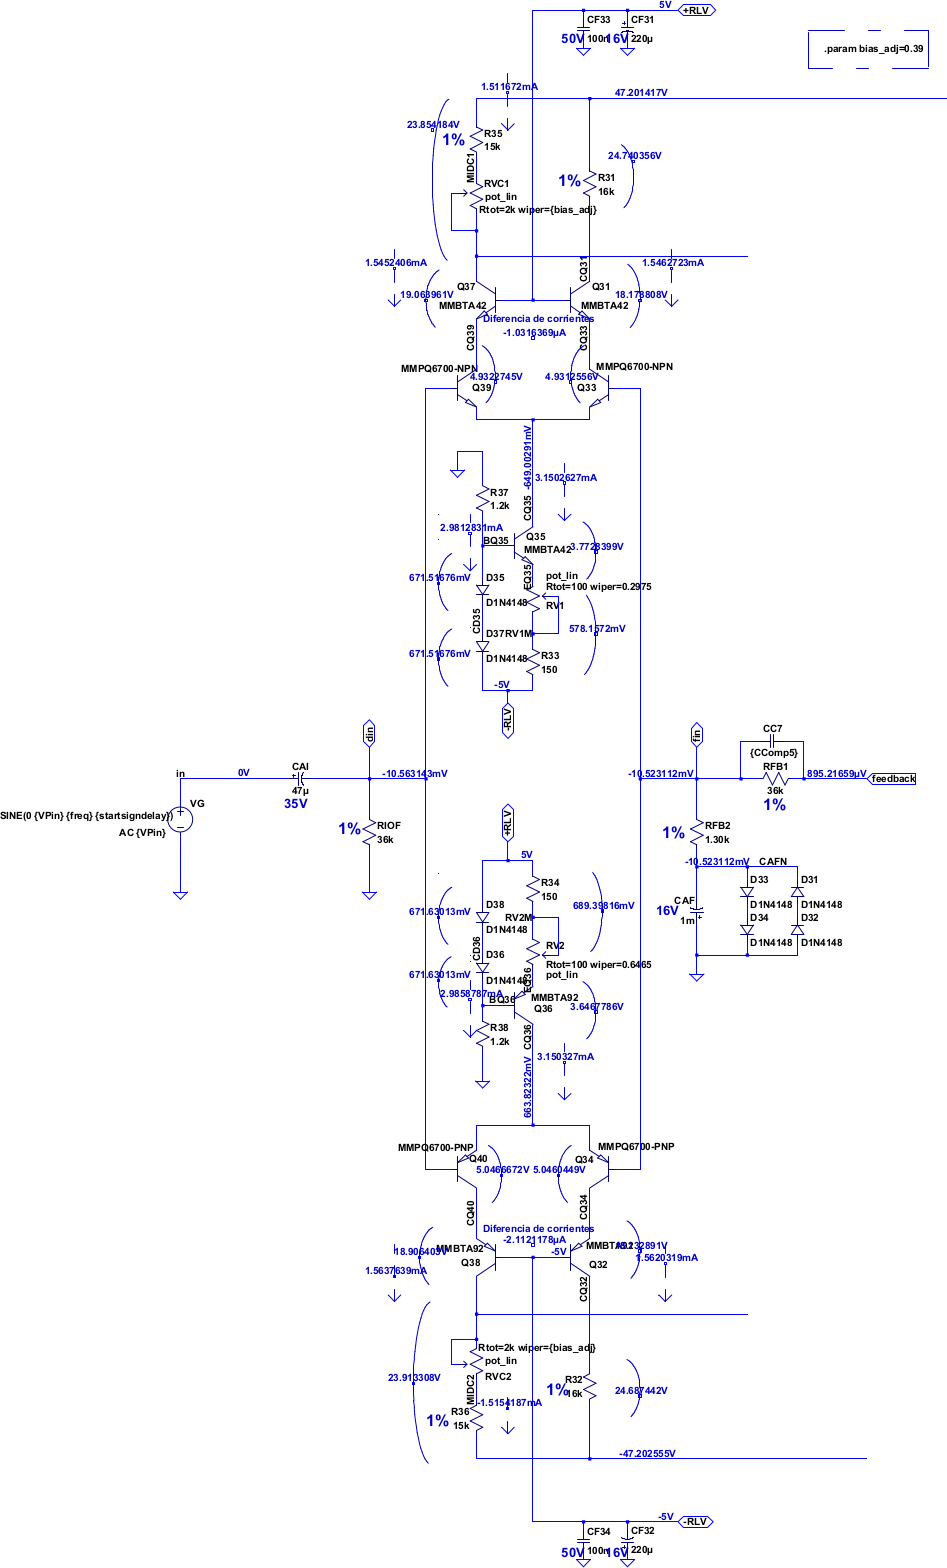
\includegraphics[width=0.36\textwidth]{img/etapa-1.png}
%\caption{Etapa primera del circuito diseñado.}
%\label{fig:etapa-1} 
%\end{figure}


\clearpage


\subsection{Etapa de amplificación de tensión}

Se optó por una configuración \textbf{CC-EC}, una para cada salida del doble par diferencial, figura~\figref{fig:vas-1}. El colector común cumple la función de ofrecer una resistencia alta a la primera etapa, independizando la polarización de los parámetros variables de los transistores de la segunda etapa. Además, aumenta la diferencia de tensión de polarización requerida entre el riel y la entrada de la etapa, lo que permite el uso de una resistencia de carga mayor en la primera etapa, mejorando su ganancia. Esta configuración, además, ofrece un alto grado de independencia de las variaciones de tensión del riel, pues todas las tensiones involucradas varían en conjunto (la única que no lo hace es masa, pero está conectada al colector de $Q_{17}$ y $Q_{18}$, nodos de alta impedancia). 


\begin{wrapfigure}{R}{0.42\textwidth}
  \begin{center}
   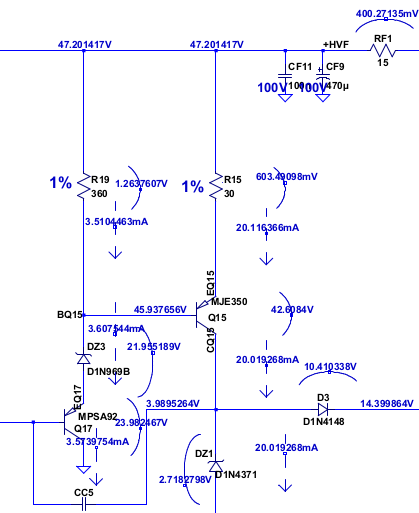
\includegraphics[width=0.4\textwidth]{img/vas-1.png}
   \caption{\textbf{VAS} en \textbf{CC-EC} del riel positivo del circuito diseñado (el otro \textbf{VAS} es perfectamente complementario).}
   \label{fig:vas-1} 
  \end{center}   
\end{wrapfigure}



%\begin{figure}[H]
%\centering
%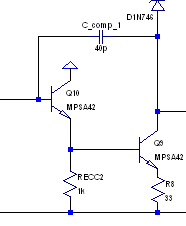
\includegraphics[width=0.3\textwidth]{img/sim/vas-1}
%\caption{VAS en CC-EC del riel negativo del circuito diseñado.}
%\label{fig:vas-1} 
%\end{figure}

Las resistencias de emisor de los \textbf{EC}, $R_{15}$ y $R_{16}$, implementan realimentaciones locales que estabilizan la corriente de polarización y ganancia de la etapa. Son realimentaciones \textbf{serie-serie} (muestrean corriente y suman tensión), estabilizando la transconductancia de la etapa. Son de valor reducido pues al estabilizar la ganancia, la reducen. Además, la caída de tensión en estas resistencias reduce la máxima excursión de la etapa antes de que saturen los transistores al mismo tiempo que determinan la corriente de colector. Se eligieron los valores exactos (junto con los de las cargas de la primera etapa) para que la corriente de polarización sea $20 \si[per-mode=symbol]{\milli\ampere}$.

Las resistencias $R_{19}$ y $R_{20}$ aseguran una corriente de polarización del colector común $3.5 \si[per-mode=symbol]{\milli\ampere}$. De no existir, la polarización podría ser muy baja, y dependiente de las variabilidades del $\beta$ del transistor del \textbf{EC}. Esta baja corriente implicaría, además, un $r_{d}$ grande, y esto es indeseable: El \textbf{EC} es un amplificador de conductancia y, como tal, funciona mejor recibiendo una señal de entrada de baja impedancia por su base.


En este punto es adecuado explicar el circuito pasa-bajos que se encuentra en los rieles de tensión alta que alimentan la primer y segunda etapa, estos simples pasa-bajos formados por un resistor y un par de capacitores, $RF_{1}$ con $CF_{9}$ y $CF_{11}$ en el riel positivo y $RF_{2}$ con $CF_{10}$ y $CF_{12}$ en el negativo, filtran el ripple de la fuente de alimentación (de $100 \si[per-mode=symbol]{\hertz}$), para eso el capacitor electrolítico de $470 \si[per-mode=symbol]{\micro\farad}$, que junto al resistor tienen una frecuencia de corte de $22.6 \si[per-mode=symbol]{\hertz}$, el capacitor cerámico de $100 \si[per-mode=symbol]{\nano\farad}$ está para filtrar el ruido de alta frecuencia que pueda filtrarse por los rieles de alimentación, principalmente debido a efectos causados por el switcheo de la etapa de salida. En general este filtrado reduce considerablemente el rechazo de de ripple de la fuente y también comprobamos que reduce un poco la distorsión, esto último es mas difícil de explicar.


\clearpage


\subsection{Multiplicador de $V_{be}$}


Se diseñó (figura~\figref{fig:mvbe}) con dos transistores para mantener la simetría total del circuito. La corriente de polarización de los transistores del VAS es $\cong 25 \si[per-mode=symbol]{\milli\ampere}$, y esta puede tener una excursión máxima de aproximadamente $4 \si[per-mode=symbol]{\milli\ampere}$ pico-a-pico. Es decir, el multiplicador debe lograr polarizarse con corrientes de $\cong 20 \si[per-mode=symbol]{\milli\ampere}$. Las simulaciones muestran que se logra una mayor estabilidad en la tensión si los transistores están polarizados con corrientes bajas. Por lo tanto, se eligió \texttt{Rmvbe} tal que consuma una corriente $< 20 \si[per-mode=symbol]{\milli\ampere}$, pero del orden de los $\si[per-mode=symbol]{\milli\ampere}$. Se podría haber elegido un valor más cercano a $20 \si[per-mode=symbol]{\milli\ampere}$, pero una simulación remplazando al multiplicador por un generador de tensión ideal mostró que el funcionamiento y la distorsión del circuito no se veían afectados. 


\begin{wrapfigure}{R}{0.42\textwidth}
  \begin{center}
   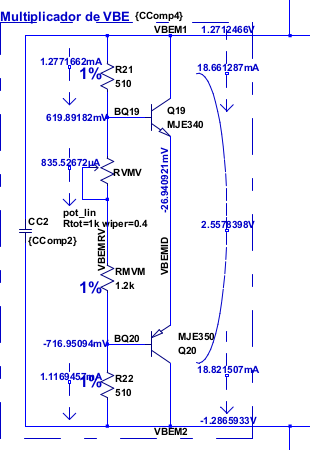
\includegraphics[height=0.5\textwidth]{img/mvbe.png}
   \caption{Multiplicador de $V_{be}$ simétrico utilizado.}
   \label{fig:mvbe}  
  \end{center}   
\end{wrapfigure}


Por esta misma razón, no se agregaron resistencias adicionales en los colectores, que usualmente se usan para generar una caída que compense el incremento de tensión con la corriente. Puede hacerse como posible optimización.

Las resistencias $R_{21}$ y $R_{22}$ se eligieron iguales por simetría, y de valor tal que la tensión generada sea levemente superior a $2.8 \si[per-mode=symbol]{\volt}$. Esto permite colocar a los transistores de salida en modo levemente \textbf{A-B}, reduciendo la distorsión de su etapa.




%\begin{figure}[H]
%\centering
%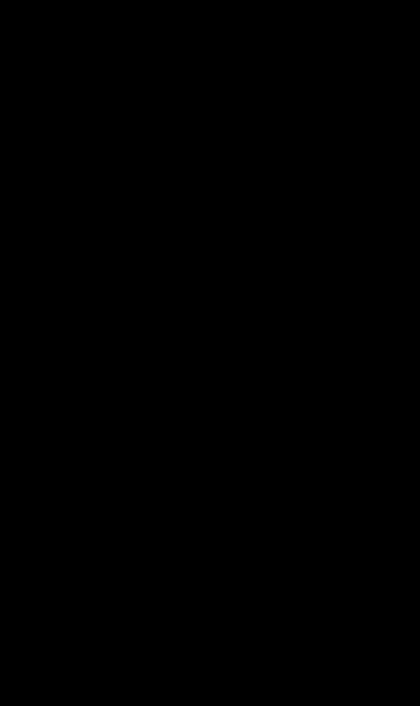
\includegraphics[height=0.5\textwidth]{img/sim/mvbe}
%\caption{Multiplicador de $V_{be}$ simétrico utilizado.}
%\label{fig:mvbe} 
%\end{figure}

%Dice en la consigna que acá toca:
%1.Explora distintos circuitos y analiza CORRECTAMENTE su funcionamiento*
%2.Calcula CORRECTAMENTE TODOS los componentes de circuitos individuales y las
%condiciones de funcionamiento*
%3.Investiga y selecciona los componentes
%4.Valida y optimiza el diseño mediante simulaciones y mediciones, y determina todos los
%parámetros de funcionamiento de los circuitos
%5.Determina si las especificaciones del circuito son alcanzables*
%6.Realiza las simulaciones, indica y explica los circuitos simulados, los puntos de medición,
%los parámetros utilizados y los resultados obtenidos
%7.Realiza mediciones, indica y explica los circuitos implementados, las mediciones
%realizadas, los instrumentos utilizados y los resultados obtenidos*
%8.Realiza los diagramas esquemáticos con las referencias de todos sus componentes
%9.Realiza el listado de componentes indicando referencia, descripción, valor, parámetros, fabricantes y posibles proveedores para cada componente.








\subsection{Etapa de salida}

Se usan transistores en configuración Darlington, para tener una ganancia de corriente elevada, y con transistores en paralelo en la parte de mayor potencia para repartir la corriente y disminuir la disipación en cada uno. Se colocaron las resistencias \texttt{R14}, \texttt{R15}, \texttt{R16} y \texttt{R17} de valor $0.1\Omega$ para ayudar a que se reparta de forma equilibrada la potencia entre los transistores de potencia \texttt{Q1}-\texttt{Q11} y \texttt{Q7}-\texttt{Q12}.




\subsection{Realimentador}

Como se había mencionado en el diseño conceptual, el factor de realimentación queda definido por las especificaciones de sensibilidad y potencia RMS que definen la ganancia. Para nuestras especificaciones, la ganancia del amplificador debe ser de $29dB$ y por lo tanto el realimentador debe atenuar $-29dB$. Se implementa mediante un divisor de tensión que muestrea tensión y suma tensión. Deben ser resistencias lo suficientemente altas para que no afecten la salida al muestrear. Con una carga de $8\Omega$, esto es sencillo. Por otra parte, la corriente que entra a la base del par diferencial de la primera etapa debe ser despreciable frente a la que circula por el realimentador para no afectar al factor $f$. Los valores usados se ven en la figura~\ref{fig:realimentacion-global}.

\begin{figure}[H]
	\centering
	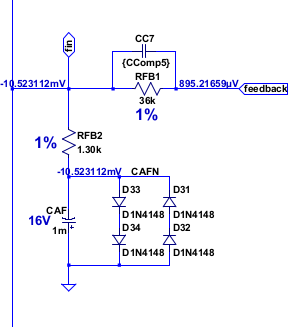
\includegraphics[width=0.4\textwidth]{img/realimentacion-global}
	\caption{Realimentación global implementada, junto con su compensación por atraso de fase.}
	\label{fig:realimentacion-global}
\end{figure}
 
 El capacitor \texttt{C1} cumple la función de modificar la realimentación en continua, a un factor unitario, y generar una simetría en las resistencias que ven las bases de los pares diferenciales de la primera etapa, y así reducir la tensión de offset. Por esta misma razón, la resistencia en paralelo a la entrada \texttt{R12}, que permite la polarización de \texttt{Q17} y \texttt{Q20} es del mismo valor que \texttt{R11}.
 

Consideremos el diagrama de la figura~\ref{fig:ampli_realimentacion}. Para hallar los valores de impedancia de entrada y salida, primero debemos reflejar las resistencias $R_{10}$ y $R_{11}$, como vemos en el siguiente dibujo.

\begin{figure}[H]
	\centering
	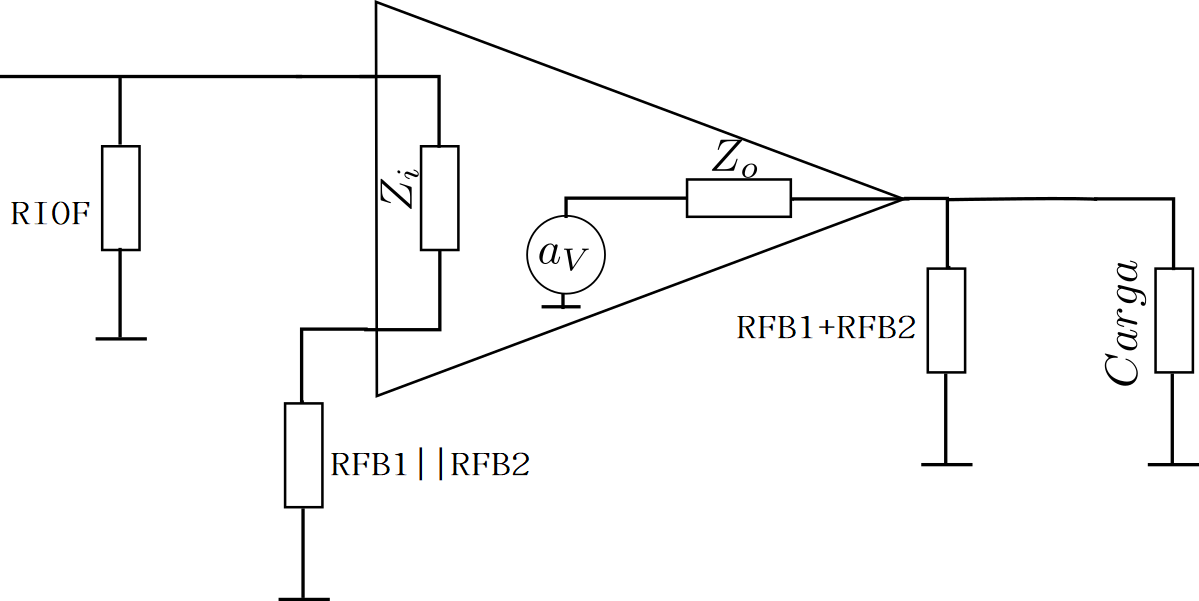
\includegraphics[width=0.5\textwidth]{img/reflejo}
	\caption{Modelo amplificador-reflejando resistencias}
	\label{fig:ampli_reflejo}
\end{figure}

Este amplificador tiene una amplificación de tensión a lazo abierto, de aproximadamente $90$ dB, con una impedancia de salida de aproximadamente $6\;\Omega$.
La realimentación tiene un valor de $\frac{1}{f} = \frac{R_{10}}{R_{10} + R_{11}} \rightarrow f = 0.035$, resultando $1+a_V\times f = 9\mathrm{K} \times 0.035 = 318.77$. La ganancia a lazo cerrado es $A\cong f^{-1} =28.6$. En cuanto a la impedancia de entrada, $R_{11}$ y $R_{10}$ se reflejan en paralelo entre ellas, en serie a la impedancia de entrada del amplificador $Z_i$. Dada la relación entre las resistencias, $R_{11}$ resulta despreciable, y a su vez, $R_{10}$ resulta despreciable en serie con $Z_i$, que resulta despreciable, en paralelo con $R_{12}$, de $10\; \mathrm{K}\Omega$. Para la resistencia de salida, tenemos la resistencia reflejada $R_{10} + R_{11}$, que es despreciable en paralelo con $Z_o || R_{Carga} = 3.42\; \Omega$. Luego $\frac{3.42}{(1 + a_V \times f)} = 0.01\; \Omega$, que es la impedancia de salida resultante. La impedancia de entrada incrementada en la ganancia de lazo resulta ser mucho mayor a $10k\Omega$. En nuestro circuito, la resistencia \texttt{R12} de valor $10k\Omega$ en paralelo a la entrada del amplificador a lazo cerrado que domina la impedancia de entrada final.






\subsection{Compensación}

Un sistema realimentado puede sufrir de pérdidas de estabilidad debido al desfasaje que se produce en la señal. Si para algunas frecuencias se produce una inversión de fase y la ganancia es unitaria o mayor entonces el sistema pasa a estar realimentado positivamente para dichas frecuencias y oscila o se desestabiliza.

Para analizar la estabilidad del sistema es necesario analizar la ganancia a lazo abierto $T(j\omega)$. Un sistema adquiere la capacidad de oscilar si para una frecuencia dada $\omega_k$ se da que $T(j\omega_k)=-1$ y se vuelve inestable si $\left| T(j\omega_k) \right| > 1 \; \land \; \angle T(j\omega_k) < -180º$.

Para esta clase de análisis es útil trazar el bode de la ganancia de lazo e identificar el margen de ganancia (MG) y de fase (MF), ver figura \ref{fig:margenes}.


\begin{figure}[H]
	\centering
	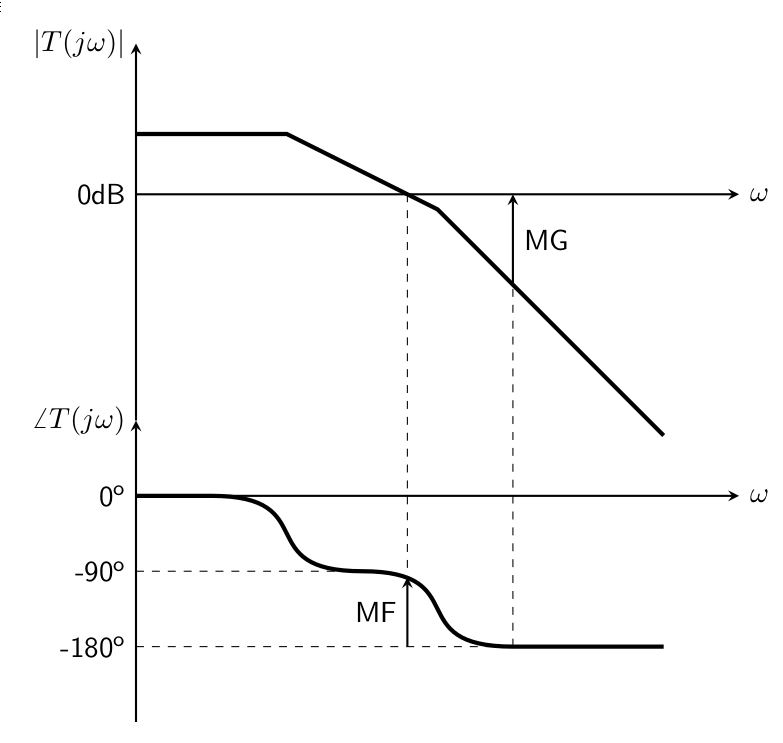
\includegraphics[height=0.4\textwidth]{img/margenes}
	\caption{Bode - margen de fase y ganancia.}
	\label{fig:margenes}
\end{figure}


Lo que representan estos margenes es lo siguiente:


\begin{description}
	\item[Margen de Ganancia] \hfill \\
		Representa la ganancia que habría que agregar (sumar en caso de dB) para volver inestable al sistema, se mide entonces la diferencia entre 0dB y la ganancia para la frecuencia en que la fase se invierte 180º. Si $\mathrm{MG} \le \mathrm{0dB}$ entonces el sistema es inestable.

	\item[Margen de Fase] \hfill \\
		Es el defasaje que habría que agregar al sistema para volverlo inestable, se mide entonces el ángulo que le resta a la fase por llegar a -180º al tener ganancia unitaria.
\end{description}

Si el margen de fase o ganancia son muy bajos o negativos, es necesario corregir, modificar el circuito para que no haya una inversión de fase en ninguna frecuencias que se amplifique en el lazo, por medio de su compensación.


Se realizó nuevamente una simulación a lazo abierto de forma análoga a la descripta en la sección anterior (figura~\ref{fig:ala}): agregando un capacitor de $1F$ en la entrada inversora del amplificador, y midiendo a la salida. Luego, a la salida se la multiplicó por $f$ para obtener una simulación de la ganancia de lazo (figura~\ref{fig:bode-la-sin-comp})

\begin{figure}[H]
	\centering
	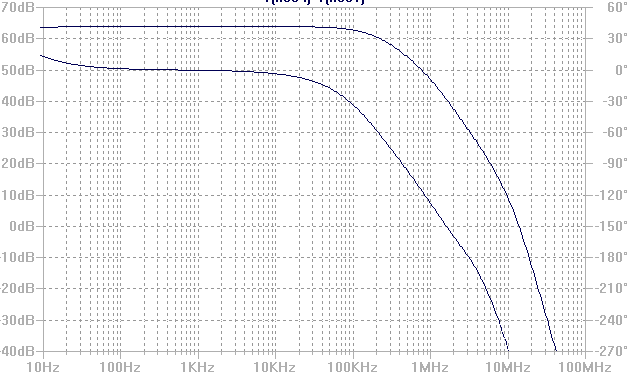
\includegraphics[height=0.4\textwidth]{img/sim/bode-la-sin-comp}
	\caption{Bode de la ganancia de lazo sin compensación. La línea inferior corresponde a la fase y la superior a la amplitud.}
	\label{fig:bode-la-sin-comp}
\end{figure}

Se puede apreciar un margen de fase negativo que es necesario compensar. El polo dominante se ubica en $180kHz$ y corresponde al nodo entre la segunda y tercera etapa: a los colectores de \texttt{Q14} y \texttt{Q9}. El margen de ganancia es de $\cong 30dB$. Desplazando al polo dominante una década y media hacia las frecuencias más bajas (hasta $5.7k\Omega$) se llega a un margen de ganancia nulo, pues un polo hace decaer la ganancia en $20dB$ por década. Sin embargo, el polo correspondiente a los nodos de entrada de la segunda etapa (bases de \texttt{Q10} y \texttt{Q13}) puede desplazarse a $5.7kHz$ con capacidades de menor valor, casi sin desplazar el polo en $180kHz$, aprovechando el efecto Miller. 
La resistencia de estos nodos está dominada por la de carga de los pares diferenciales (\texttt{RC1} y \texttt{RC2}), de valor $2.4k\Omega$. Siendo $\frac{1}{2 \pi RC}$ la frecuencia del polo, se obtiene $C\cong 11nF$. Ahora bien, si la capacidad se coloca, en vez de contra masa, contra la salida de la etapa (colectores de \texttt{Q14} y \texttt{Q9}), se puede usar una capacidad desde $20pF$, pues recordemos que la etapa tiene una amplificación de alrededor de $55dB$ o 560 veces. 

Se partió de ese valor como piso, se fue ajustando por simulación, y finalmente se colocaron capacitores (\texttt{C\_comp\_1} y \texttt{C\_comp\_2}) de $40pF$. Esto da un margen de fase de $85^{\circ}$ y un ancho de banda de $2.4MHz$. Estos capacitores limitan el slew rate, pero se observó que para valores menores a $100pF$ el slew rate se encontraba por arriba de los $7.5\frac{V}{\mu s}$ necesarios para el ancho de banda de potencia especificado, y para valores menores a $60pF$, sobre los $15V/\mu s$ especificados. Por otra parte, incrementar este capacitor reduce la ganancia de lazo en frecuencias altas y, por lo tanto, los beneficios que esto trae a la distorsión, resistencias de entrada y salida, etc. Se optó por un valor de capacidades, con margen, que podría eventualmente reducirse.

Luego, se agregó un capacitor en paralelo al realimentador (\texttt{C\_comp\_3}) para mejorar levemente estas especificaciones. Esto agrega un cero seguido de un polo. Por ejemplo, para la frecuencia del cero, la fase se incrementa en $45^{\circ}$ y la ganancia aumenta sólo en $3dB$, por lo que el ancho de banda se verá incrementado levemente y el margen de fase significativamente. Se comprobó simulando que ubicar el cero en $4MHz$ es un buen valor. Esto se obtiene con una capacidad de $4pF$ pues $\frac{1}{2 \pi 10k\Omega 4pF}\cong 4MHz$. El bode resultante de la ganancia de lazo compensado se muestra en la figura~\ref{fig:bode-la-con-comp}

\begin{figure}[H]
	\centering
	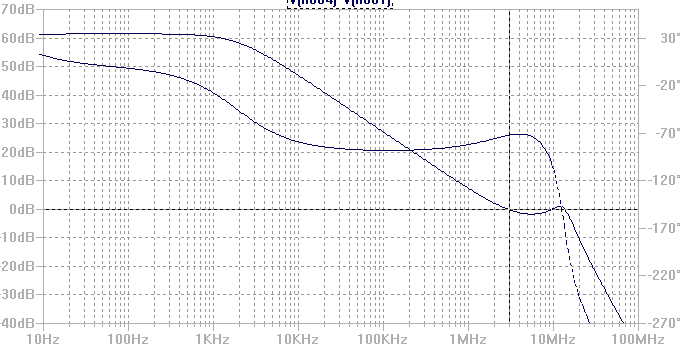
\includegraphics[height=0.4\textwidth]{img/sim/bode-la-con-comp}
	\caption{Bode de la ganancia de lazo con compensación. La línea punteada corresponde a la fase y la llena a la amplitud.}
	\label{fig:bode-la-con-comp}
\end{figure}


El margen de fase resultante ese de $105^{\circ}$ y el ancho de banda de $3MHz$, con un margen de ganancia de $3dB$. Se puede ver en la figura~\ref{fig:slew} que la respuesta al escalón no oscila.

Otra compensación se implementó para corregir el comportamiento inductivo del multiplicador de $V_{be}$ en altas frecuencias. Se compensó con el capacitor \texttt{C\_mvbe\_comp} de $20nF$.

Finalmente, con las ganancias a lazo abierto y lazo cerrado, realizamos el siguiente diagrama:

\begin{figure}[H]
	\centering
	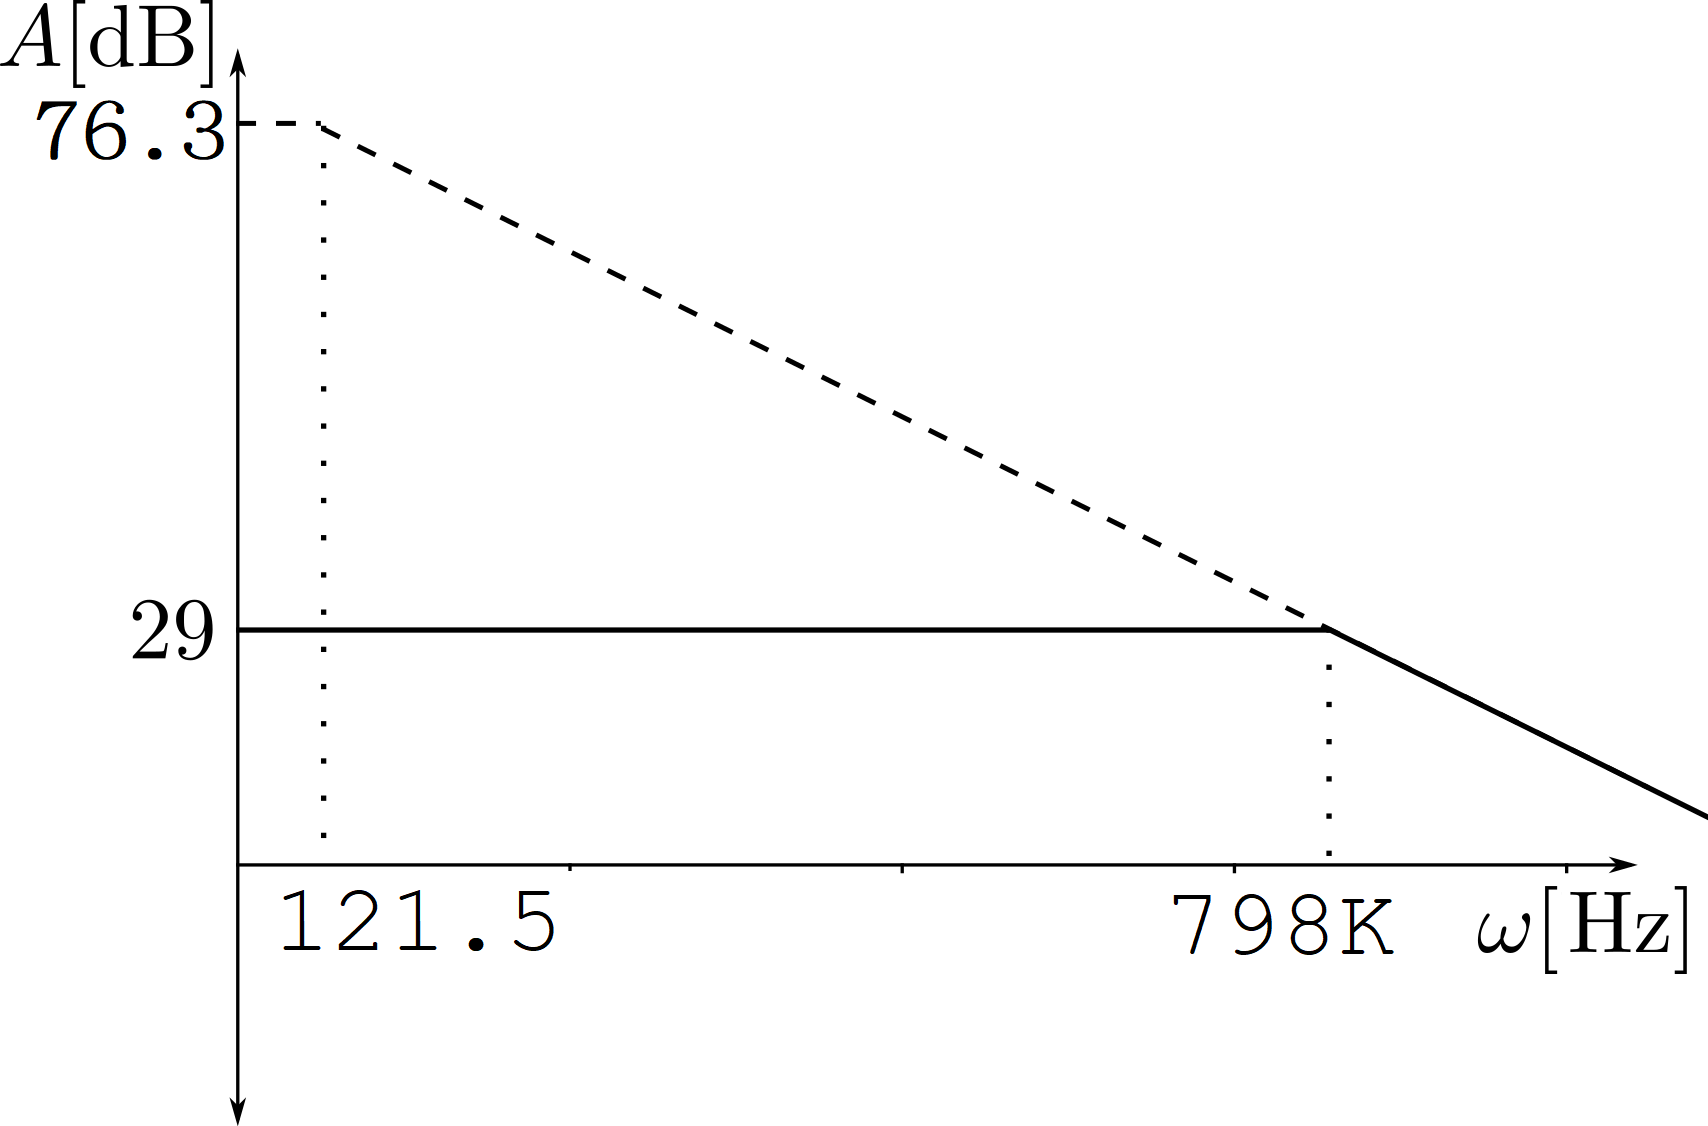
\includegraphics[width=0.5\textwidth]{img/bodecompensado}
	\caption{Aumento del ancho de banda, debido a la realimentación.}
	\label{fig:bode-copmensado}
\end{figure}

Como se puede ver en el gráfico, la ganancia a lazo abierto, de $90$ dB, tiene un ancho de banda de $1.8kHz$, totalmente inútil para un amplificador de audio que trabaja con señales de decenas de kilohertz. Cuando aplicamos la realimentación, la ganancia cae a $29$ dB, pero la frecuencia de corte pasa a ser $1.8kHz \times (1 + a_V \times f) = 1.8 \times 1107 = 1.9 \mathrm{MHz}$.